% -*- coding: utf-8 -*-
% !TEX encoding = UTF-8 Unicode
% !TEX root =  main.tex

\chapter{Grundlagen der Vektorregelung}
\label{cha:Grundlagen der Vektorregelung}

%% -- Einführung in die Vektorregelung
In modernen Antriebssystemen ist es häufig unerlässlich, entscheidende Maschinengrößen wie Drehzahl oder Drehmoment auf einen gewünschten Wert einzustellen.
Dabei kamen der Vergangenheit häufig Gleichstrommaschinen zum Einsatz, welche sich durch gute Regel- und Einstelleigenschaften bei den geforderten Parametern auszeichnen.
Große Fortschritte in den Bereichen der Leistungselektronik und Reglerkomponenten führen dazu, dass Antriebe wesentlich einfacher mit Synchronmaschinen realisiert werden können.
Dabei haben Drehfeldmaschinen, aufgrund fehlender mechanischer Kommutation den Vorteil, dass kein nennenswerter Verschleiß Auftritt.

Entscheidend für den Aufbau einer geregelten PMSM ist die Vektor- bzw. feldorientierte Regelung. 
Die Maschine wird näherungsweise mit sinusförmigen Strömen gespeist. 
Ebenso besitzen alle weiteren auftretenden elektrischen Größen wie Spannungen, Flüsse oder Felder aufgrund ihres Zeitverhaltens annähernd Sinusform \parencite[S.~1]{nuss2010}.	
Die Idee der Vektorregelung ist es nun, nicht die zeitlichen Momentanwerte der Ströme zu verändern, sondern die erfassten Wechselgrößen in ein Zwei-komponentiges rotierendes Koordinatensystem zu übertragen.
Diese Komponenten werden regelungstechnisch verwertet und zurück transformiert.

\section{Raumzeigerdarstellung}
\label{sec:raumzeiger}

Die stationären Zusammenhänge der elektrischen Größen in der Maschine, welche ursächlich aus dem Zusammenhang von $\Psi$ und B herrühren, können zunächst mithilfe komplexer Zeitzeiger beschrieben werden. Dabei lassen sich die Statorströme, $i_{s,1}$, $i_{s,2}$, und $i_{s,3}$ einer Drehfeldmaschine mit idendischer Amplitunde $\hat i_{s}$ und Statorkreisfrequenz $\omega_{s}$  und einer jeweiligen $120^\circ$ Phasenverschiebung als

\begin{align}
	\begin{split}
	i_{s,i} = Re\{\underline{i}_{s,i}\} = Re\{\underline{\hat i}_{s,i}\cdot e^{j\omega_{s}t}\} = Re\Bigl\{\hat{i_{s}}\cdot e^{j(\omega_{s}t+0-(i-1)\cdot\tfrac{2\pi}{3})}\Bigr\}
	\\= \hat{i}_{s}\cdot cos\bigg(\omega_{s}t+\varphi_{0}-(i-1)\cdot\frac{2\pi}{3}\bigg)~;~mit~i=1,2,3 \label{statorströme} 
\end{split}
\end{align}

mit den komplexen Zeitzeigern

\begin{align}
	\underline{i}_{s,i} = \underline{\hat i}_{s,i}\cdot e^{j\omega_{s}t}~;~mit~i=1,2,3 \label{zeitzeiger}
\end{align}

und den komplexen Amplituden

\begin{align}
	\underline{\hat i}_{s,i} = \hat{i_{s}}\cdot e^{j(\omega_{s}t+0-(i-1)\cdot\tfrac{2\pi}{3})}~;~mit~i=1,2,3 \label{amplituden}
\end{align}

darstellen. 
Die folgende Abbildung \ref{fig:zeitzeiger} veranschaulicht die vorangegangenen Gleichungen \ref{statorströme}, \ref{zeitzeiger} sowie \ref{amplituden} und stellt beispielhaft den Zeitzeiger $i_{s,1}$ dar.

\begin{figure}[h]
	\centering
	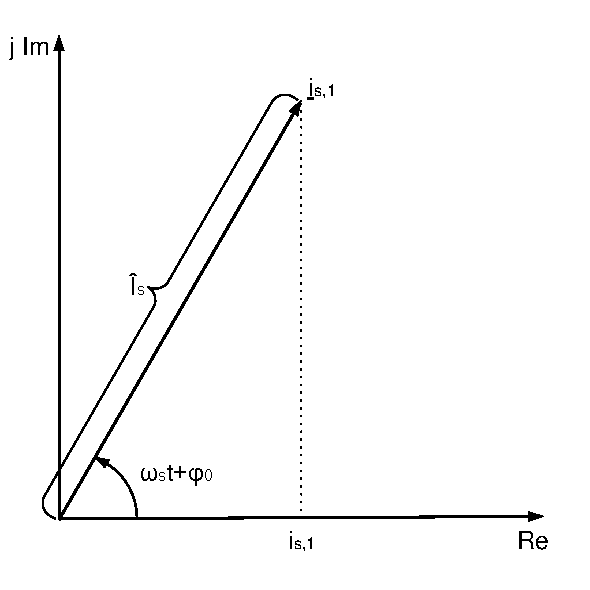
\includegraphics[width=0.5\textwidth]{zeitzeiger.pdf}
	\label{fig:zeitzeiger}
	\caption{Beispielhafte Lage eines Zeitzeigers.}
\end{figure}

Da das Ziel darin besteht, den dynamischen Rotationsvorgang einer PMSM zu modellieren, ist die Verwendung eines Zeitzeigers, mit dem nur stationöre Vorgänge beschrieben werden können, nicht angebracht. 
Hier ist es Zweckmäßig, einen Operator so zu entwickeln, dass dieser in der Lage ist, dynamische Vorgänge zu beschrieben, ohne dazu Nebenbedingungen wie beispielsweise die Periodizität heranzuziehen. 
Bei der Entwicklung bieten sich die Statorphasenströme $i_{s,1}$, $i_{s,2}$, und $i_{s,3}$ des Dreiphasensystems an.
Diese stehen zu jedem Zeitpunkt zur Verfügung. 
Es sei angemerkt, dass dabei die Nullbedingung erfüllt ist. 
Die Summe der Statorphasenströme muss immer null sein, was beim Einsatz von Drehfeldmaschinen idr. gegeben ist.
Dadrurch ist es auch immer möglich mit Kenntnis zweier Größen auf die Dritte zu schließen, da gilt:

\begin{align}
	i_{s,1} + i_{s,2} + i_{s,3} = 0 
	\label{knotengleichung}
\end{align}


Nun ist der zweikomponentige Zeitzeiger immer um mindestens zwei Momentanwerte erweiterbar. 
Ein hierfür geeigneter Ansatz zur Erzeugung eines Raumzeigers wurde erstmals in kovacs1959 veröffentlicht:

\begin{align}
	\underline{i}_{s}(t) = \frac{2}{3} \cdot \Bigl\{\underline{i}_{s,1}(t) + \underline{i}_{s,2}(t)\cdot e^{j\tfrac{2\pi}{3}} + \underline{i}_{s,3}(t)\cdot e^{j\tfrac{4\pi}{3}} \Bigr\} \label{statorstromzeiger}
\end{align}

Um jetz aufzeigen zu können, dass der Ansatz aus \ref{statorstromzeiger} im stationären Zustand mit dem entsprechenden Statorstromzeitzeiger übereinstimmt und schlussendlich den Raumzeiger zu erzeugen, werden zunächst in \ref{statorstromzeiger} die Statortrommomentanwerte aus \ref{statorströme} eingesetzt.
Dadurch erhält man

\begin{align}
\underline{i}_{s}(t) = \frac{2}{3} \cdot \biggl\{\hat{i}_{s}\cdot cos(\omega_{s}t+\varphi_{0}) + \hat{i}_{s}\cdot cos\bigg(\omega_{s}t+\varphi_{0}-\frac{2\pi}{3}\bigg)\cdot e^{j\tfrac{2\pi}{3}} + \hat{i}_{s}\cdot cos\bigg(\omega_{s}t+\varphi_{0}-\frac{4\pi}{3}\bigg)\cdot e^{j\tfrac{4\pi}{3}} \biggr\}
\label{zwischen1}
\end{align}

Wird nun die trigonometrische Cosinus-Funktion durch die entsprechende exponentielle Darstellung ersetzt, folgt hieraus

\begin{align}
	\begin{split}
	\underline{i}_{s}(t) = \frac{2}{3} \cdot \hat{i}_{s} \cdot \biggl\{ \frac{1}{2} \cdot ( e^{j(\omega_{s}t+\varphi_{0})} + e^{-j(\omega_{s}t+\varphi_{0})} ) + \frac{1}{2} \cdot ( e^{j(\omega_{s}t+\varphi_{0}-\frac{2\pi}{3})} + e^{-j(\omega_{s}t+\varphi_{0}-\frac{2\pi}{3})})\cdot e^{j\tfrac{2\pi}{3}} + \\ \frac{1}{2} \cdot ( e^{j(\omega_{s}t+\varphi_{0}-\frac{4\pi}{3})} + e^{-j(\omega_{s}t+\varphi_{0}-\frac{4\pi}{3})})\cdot e^{j\tfrac{4\pi}{3}}  \biggr\}
	\label{zwischen2}
	\end{split}
\end{align}

Nach ausmultiplizieren der Terme folgt mit $1+e^{j\tfrac{4\pi}{3}}+e^{j\tfrac{8\pi}{3}}=0$ das Ergebnis und somit der Raumzeiger

\begin{align}
	\underline{i}_{s} = \frac{2}{3} \cdot \hat{i}_{s}\cdot\biggl\{ \frac{3}{2} \cdot  e^{j(\omega_{s}t+\varphi_{0})} + \frac{1}{2} \cdot e^{-j(\omega_{s}t+\varphi_{0})} \cdot \bigg( 1+e^{j\tfrac{4\pi}{3}}+e^{j\tfrac{8\pi}{3}} \bigg)  \biggr\} = \hat{i}_{s} \cdot e^{j(\omega_{s}t+\varphi_{0})}
	\label{zeigerende}
\end{align}

Das Ergebnis von \ref{zeigerende} entspricht strukturell dem in \ref{statorströme} angegebenen Statorstromzeitzeiger. 
Dadurch ist sichergestellt, dass der Ansatz aus \ref{statorstromzeiger} in der Lage ist als Gesamtzeiger, bestehend aus den Momentanwerten der Statorströme, zu fungieren. 
Die folgende Abbildung \ref{fig:raumzeigermaschine} zeigt zur Veranschaulichung eine zweipolige Drehfeldmaschine mit zugehörigem Zeigerdiagramm, welches den Statorstromraumzeiger beinhaltet. 

\begin{figure}[h]
	\centering
	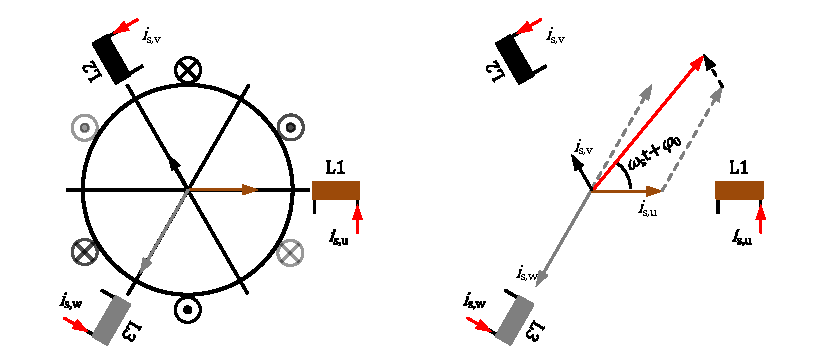
\includegraphics[width=0.5\textwidth]{raumzeigermaschine.pdf}
	\label{fig:raumzeigermaschine}
	\caption{zweipolige Drehfeldmachine mit beispielhafter Statorstromraumzeigerlage}
\end{figure}

Mit der Einführung des Raumzeigers ist die theoretische Grundlage dafür geschaffen, die PMSM mit einer feldorientierten Regelung zu versehen. 
Da sich, wie Eingangs beschrieben, alle Größen in der Drehfeldmaschine näherungsweise sinusförmig verhalten, ist die Stromraumzeigerdarstellung aus \ref{statorstromzeiger} für alle andren dreiphasigen Größen als allgemeine Raumzeigerdarstellung definierbar.

\begin{align}
	\underline{a}(t) = \frac{2}{3} \cdot \Bigl\{\underline{a}_{1}(t) + \underline{a}_{2}(t)\cdot e^{j\tfrac{2\pi}{3}} + \underline{a}_{3}(t)\cdot e^{j\tfrac{4\pi}{3}} \Bigr\} \label{raumzeigerdefinition}
\end{align}

Im Folgenden werden die in der Praxis benötigten Transformationsvorschriften erläutert, welche das Wechseln zwischen Phasen- und Raumzeigergrößen erlauben.


\section{Beschreibung in $\alpha$-$\beta$-Koordinatensystem}\label{sec:clark}

Als Grundlage für das Wechseln zwischen Phasen- und Raumzeigergrößen dient zunächst die Definition aus \ref{raumzeigerdefinition}. Die Definitionsgleichung lässt sich in Real- und Imaginärteil aufspalten. Es kommt so zu folgender Aufteilung

\begin{align}
	Re{\underline{a}(t)} = \frac{2}{3} \cdot \Bigl\{ a_{1}(t) + a_{2}(t) \cdot\cos{\frac{2 \pi}{3}} + a_{3}(t) \cdot\cos{\frac{4 \pi}{3}} \Bigr\}
	\label{realteil}
\end{align}

\begin{align}
	Im{\underline{a}(t)} = \frac{2}{3} \cdot \Bigl\{ ~~~~~~~~a_{2}(t)\cdot\sin{\frac{2 \pi}{3}} + a_{3}(t) \cdot\sin{\frac{4 \pi}{3}} \Bigr\}
	\label{imaginärteil}
\end{align}

In Zusammenhang mit der Clarke Transformationsvorschrift ist es üblich, den Realteil in $\alpha$- und den Imaginärteil als $\beta$-Koordinaten auszudrücken. 
Daher ist die Clarke Transformation im deutschsprachigen Bereich auch $\alpha$ -$\beta$-Transformation bekannt.
Um im Weiteren die in der Praxis notwendige Transformationsmatrix zu erhalten, werden die Trigonometrischen Ausdrücke numerisch dargestellt. 
Aus \ref{realteil} und \ref{imaginärteil} folgt somit

\begin{align}
	a_{\alpha}(t) = \frac{2}{3} \cdot \Bigl\{ a_{1}(t) - \frac{1}{2} \cdot a_{2}(t) - \frac{1}{2} \cdot a_{3}  \Bigr\}
	\label{alpha}
\end{align}

\begin{align}
	a_{\beta}(t) = \frac{2}{3} \cdot \Bigl\{ ~~~~~~ \frac{\sqrt{3}}{2} \cdot a_{2}(t) - \frac{\sqrt{3}}{2} \cdot a_{3}  \Bigr\}
	\label{beta}
\end{align}

Der entstandene Raumzeiger in  $\alpha$-$\beta$-Koordinaten ist in allgemeiner Forma als 

\begin{align}
	\underline{a}(t) = a_{\alpha}(t) +j a_{\beta}(t)
	\label{raumzeigeralphabeta}
\end{align}

darstellbar. Um die $\alpha$- und $\beta$-Komponente des entstandenen Raumzeigers besser nachvollziehen zu können, zeigt die Abbildung \ref{alphabetakoordinaten} eine beispielhafte Lage des Zeigers in $\alpha$-$\beta$-Koordinaten.

\begin{figure}[h]
	\centering
	
\includegraphics[width=0.5\textwidth]{alphabetakoordinaten.pdf}
	\label{fig:alphabetakoordinaten}
	\caption{Beispielhafte Lage des Raumzeigers im $\alpha$-$\beta$-Koordinatensystem.}
\end{figure}

Nachdem sich der Raumzeiger im neuern Koordinatensystem darstellen lässt, ist es nun entscheidend, eine mathematische Transformationsvorschrift aufzustellen, die sich an \ref{alpha} und \ref{beta} orientiert. 
Übertragen auf eine Vektorschreibweise lautet die Transformation

\begin{align}
	\begin{bmatrix}
	a_{\alpha} \\
	a_{\beta} 
	\end{bmatrix}
	=\underline{T^\prime}\cdot 
	\begin{bmatrix}
	a_{1} \\
	a_{2} \\
	a_{3}
	\end{bmatrix}
	\label{clarkevektor}
\end{align}

mit der Transformationsmatrix

\begin{align}
	\underline{T^\prime} = 
	\begin{bmatrix}
		1 & -\frac{1}{2} & -\frac{1}{2}  \\
		0 & ~~\frac{\sqrt{3}}{2} & ~~\frac{\sqrt{3}}{2}
	\end{bmatrix}
	\label{clarkematrix}
\end{align}

Mit dieser Matrix ist es möglich, die dynamische Drehfeldgößen eines dreiphasigen Systems auf zwei Größen zu reduzieren sowie Momentanwerte und Amplitude in einem Raumzeiger darzustellen.
Der Faktor $\frac{2}{3}$ normiert dabei $a_{\alpha}$ und $a_{\alpha}$ auf den Betrag der entsprechenden Eingangsgrößen.
Die Transvormation mit diesem Vorfaktor ist daher längeninvariant.

Für eine Regelung fehlt eine Rücktransvormationsvorschrift, mit deren Hilfe die $\alpha$- und $\beta$-Komponente wieder in ein Dreiphasensystem gebracht werden kann.
Die inverse Matrix bildet sich aus der Transformationsmatrix \ref{clarkematrix}. 
Da es sich hier aber um eine nichtquadratische Matrix handelt, ist diese zunächst nicht invertierbar.
Folglich muss die Matrix um eine Eingangsgröße erweitert werden.
Dabei bietet sich die Nullbedingung des Systems an.
Bindet man die Kontengleichung aus \ref{knotengleichung} in \ref{clarkematrix} ein, folgt für die vektorielle Transformationsbeziehung

\begin{align}
	\begin{bmatrix}
		a_{\alpha} \\
		a_{\beta} \\
		a_{0}
	\end{bmatrix}
	=\underline{T}\cdot 
	\begin{bmatrix}
		a_{1} \\
		a_{2} \\
		a_{3}
	\end{bmatrix}
	\label{clarkevektornull}
	\end{align}

mit der Transformationsmatrix

\begin{align}
	\underline{T} =
	\begin{bmatrix}
		1 & -\frac{1}{2} & -\frac{1}{2}  \\
		0 & ~~\frac{\sqrt{3}}{2} & ~~\frac{\sqrt{3}}{2} \\
		\frac{1}{2} & ~~\frac{1}{2} & ~~\frac{1}{2}
	\end{bmatrix}
	\label{clarkematrixnull}
\end{align} 

Die auf diese Art entstandene quadratische Matrix ist eindeutig invertierbar.
Daher folgt für

\begin{align}
	\begin{bmatrix}
	a_{1} \\
	a_{2} \\
	a_{3}
	\end{bmatrix}
	=\underline{T}^{-1}\cdot 
	\begin{bmatrix}
	a_{\alpha} \\
	a_{\beta} \\
	a_{0}
	\end{bmatrix}
	\label{inverseclarkevektornull}
\end{align}

die inverse Transformationsmatrix

\begin{align}
	\underline{T}^{-1} =
	\begin{bmatrix}
		~~1 & 0 & 1  \\
		-\frac{1}{2} & \frac{\sqrt{3}}{2} & 1 \\
		~~\frac{1}{2} & \frac{\sqrt{3}}{2} & 1
	\end{bmatrix}
	\label{inverseclarkematrixnull}
\end{align}

Für die Praxisanwendung reicht die vereinfachte inverse Clarke-Transformation mit der Beziehung

\begin{align}
	\begin{bmatrix}
		a_{1} \\
		a_{2} \\
		a_{3}
	\end{bmatrix}
	=\underline{T}^{-1}\cdot 
	\begin{bmatrix}
		a_{\alpha} \\
		a_{\beta} \\
	\end{bmatrix}
	\label{inverseclarkevektornulleinfach}
\end{align}
 
 und der Transformationsmatrix 
 
 \begin{align}
 	\underline{T}^{-1} =
 	\begin{bmatrix}
 		~~1 & 0   \\
 		-\frac{1}{2} & \frac{\sqrt{3}}{2}  \\
 		~~\frac{1}{2} & \frac{\sqrt{3}}{2} 
 	\end{bmatrix}
 	\label{inverseclarkematrixnulleinfach}
 \end{align}
 
 aus. 
 Da die Nullkomponente der Phasengröße null ist, kann auch $a_{0}$ null gesetzt werden, was dem Wegfall der letzten Spalte von ${T^\prime}$ entspricht.

\section{Beschreibung in rotorfesten d-q-Koordinatensystem}\label{sec:park}

Für die Regelung von Drehfeldmaschinen hat es sich als praktikabel herausgestellt, die Systembeschreibung von der im Vorfeld beschriebenen ortsfesten Koordinatensystem in ein, mit der Winkelgeschwindigkeit des Rotors, rotierendes Koordinatensystem zu überführen. 
Daher wird die Darstellung auch rotorfest genannt. 
Die Vorteile dieser Koordinatenbeschreibung liegen zum einen in einer einfacheren Darstellbarkeit elektrophysikalischer Zusammenhänge und zum anderen dass die Raumzeigergrößen näherungsweise Gleichgrößen sind.
Dadurch lassen sich klassische Regelvefahren auf die Maschine anwenden.
Das Regelverhalten ähnelt dem der Gleichstrommaschine, welche sich durch eine gute Regelbarkeit auszeichnet. 
Für die folgende Park Transformation dient die zuvor durchgeführte Clarke Transformation als Grundlage. 
Zur Verdeutlichung der Transvormationsvorschriften dient die nachfolgende Abbildung am Beispiel eines Statorstromraumzeigers

\begin{figure}[h]
	\centering
	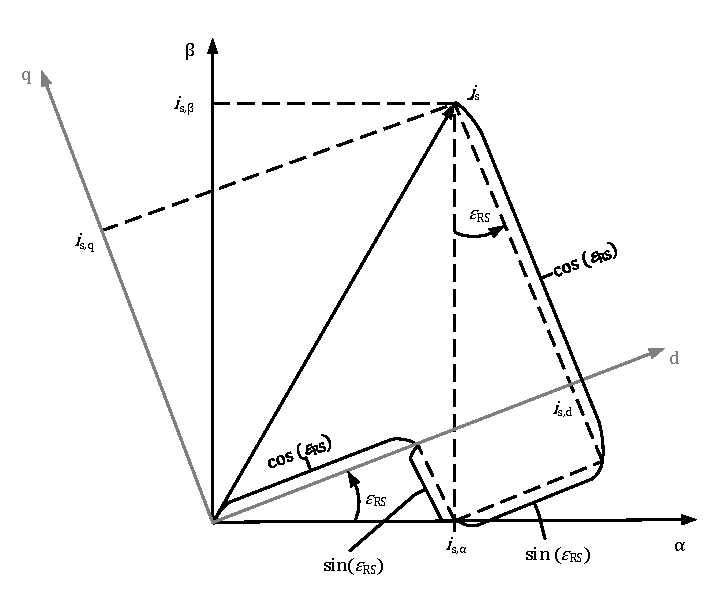
\includegraphics[width=0.5\textwidth]{dqkoordinaten.pdf}
	\label{fig:dqkoordinaten}
	\caption{Zusammenhang der $\alpha$-$\beta$-Koordinaten und der d-q- Raumzeigerkomponenten}
\end{figure}


Hier ist neben dem ortsfesten $\alpha$-$\beta$-Koordinatensystem auch das rotierende Koordinatensystem erkennbar. 
Das rotierende System wird als d-q-Koordinatensystem bezeichnet, wobei d für direct axis und q für quadrature axis steht.
Der für die Transformation entscheidende Winkel ist hier mit $\varphi_{L}$ gekennzeichnet.
Mit Hilfe der Abbildung lässt sich nun die Transformationsbeziehung zwischen $\alpha$-$\beta$-Koordinaten und d-q-Koordinaten aufstellen.

\begin{align}
	\begin{bmatrix}
		a_{d} \\
		a_{q} 
	\end{bmatrix}
	=\underline{T^\prime}\cdot 
	\begin{bmatrix}
		a_{\alpha} \\
		a_{\beta}
	\end{bmatrix}
	\label{parkvektor}
\end{align}

Die Transformationsmatrix lautet dann

\begin{align}
	\underline{T^\prime} =
	\begin{bmatrix}
		~~~\cos{\varphi_{L}} & \sin{\varphi_{L}} \\
		-\sin{\varphi_{L}} & \cos{\varphi_{L}}
	\end{bmatrix}
	\label{parkmatrix}
\end{align}

Da die Matrix um eine quadratische ist, kann diese ohne weiteres invertiert werden.
Die Rücktransformation von d-q-Koordinaten in $\alpha$-$\beta$-Koordinaten ist für die Regelung ebenfalls von entscheidender Bedeutung, um aus dem rotierenden Raumzeiger im letzten Schritt wieder die drei Phasengrößen zu erhalten. 
Es gilt für die Rücktransformation also die Beziehung

\begin{align}
	\begin{bmatrix}
		a_{\alpha} \\
		a_{\beta}
	\end{bmatrix}
	=\underline{T}^{-1}\cdot 
	\begin{bmatrix}
		a_{d} \\
		a_{q} 
	\end{bmatrix}
	\label{parkvektorinvers}
\end{align}

mit der Transformationsmatrix

\begin{align}
	\underline{T}^{-1} =
	\begin{bmatrix}
		\cos{\varphi_{L}} & -\sin{\varphi_{L}} \\
		\sin{\varphi_{L}} & ~~~\cos{\varphi_{L}}
	\end{bmatrix}
	\label{parkmatrixinvers}
\end{align}



\section{Signalflussplan der Vektorregelung}\label{sec:signalflussplan}

In diesem Abschnitt mit Hilfe der Transformationsvorschriften aus den vorherigen Abschnitten \ref{sec:clark} und \ref{sec:park} vorbereitend ein Signalflussplan entwickelt werden.
Dieser Plan soll im praktischen Teil ins Gesamtsystem integriert werden können.
Zur einfacheren Darstellung der Clarke- und Parktransformation werden zunächst entsprechende Signalflussbilder eingeführt.

\begin{figure}[h]
	\centering
	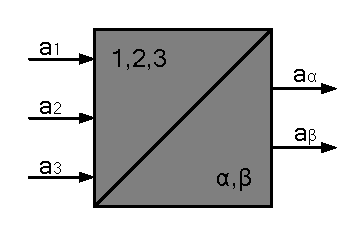
\includegraphics[width=0.5\textwidth]{blockbildclarke.pdf}
	\label{fig:blockbildclarke}
	\caption{Clarke Blockbild}
\end{figure}

Bei der Parktransformation muss der Winkel $\varphi_{L}$, um den das $\alpha$-$\beta$-Koordinatensystem zum d-q-System verschoben ist, zugeführt werden.

\begin{figure}[h]
	\centering
	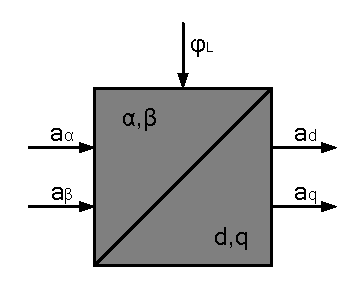
\includegraphics[width=0.5\textwidth]{blockbildpark.pdf}
	\label{fig:blockbildpark}
	\caption{Park Blockbild}
\end{figure}

Die entsprechenden Rücktransformationen werden in den folgenden zwei Abbildungen dargestellt.

\begin{figure}[h]
	\centering
	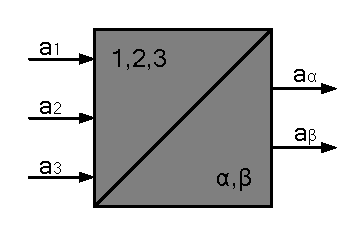
\includegraphics[width=0.5\textwidth]{blockbildclarke.pdf}
	\label{fig:blockbildinverseclarke}
	\caption{Inverse Clarketransformation Blockbild}
\end{figure}

\begin{figure}[h]
	\centering
	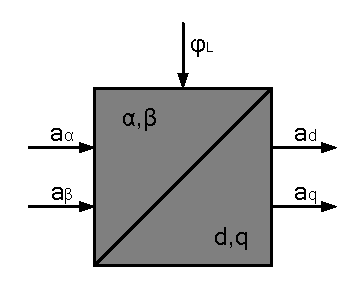
\includegraphics[width=0.5\textwidth]{blockbildpark.pdf}
	\label{fig:blockbildinversepark}
	\caption{Inverse Park-Transformation Blockbild}
\end{figure}

Mit Hilfe der Blockbilder kann jetzt die sowohl die vollständige Hintransformation eines Dreiphasensystems in ein rototorisches, zweikomponentiges Bezugsystem, als auch die entsprechende Rücktransformation, als Signalflussbild skizziert werden.

\begin{figure}[h]
	\centering
	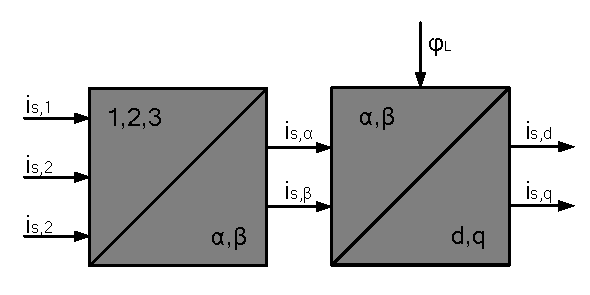
\includegraphics[width=0.5\textwidth]{blockbildclarkepark.pdf}
	\label{fig:blockbildclarkepark}
	\caption{Flussbild Clarke-Park-Transformation}
\end{figure}

Abbildung \ref{fig:blockbildclarkepark} zeigt die Transformation der Statorphasenströme $i_{s,1}$, $i_{s,2}$ und $i_{s,3}$ in d-q-Komponenten, während die nachfolgende Grafik \ref{fig:blockbildinverseclarkepark} die zusammenhängende Rücktransformation verbildlicht.

\begin{figure}[h]
	\centering
	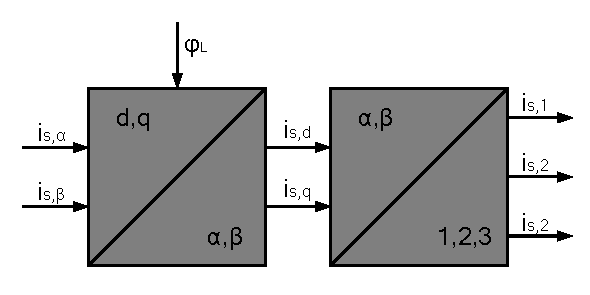
\includegraphics[width=0.5\textwidth]{blockbildinverseclarkepark.pdf}
	\label{fig:blockbildinverseclarkepark}
	\caption{Flussbild der inversen Clarke-Park-Transformation}
\end{figure}


 
%%% Local Variables: 
%%% mode: latex
%%% TeX-master: "main"
%%% TeX-open-quote: "\\enquote{"
%%% TeX-close-quote: "}"
%%% LaTeX-csquotes-open-quote: "\\enquote{"
%%% LaTeX-csquotes-close-quote: "}"
%%% End: 
